\section{\label{Geometry}幾何学モデリング}
\markright{\arabic{section}. 幾何学モデリング}

Euslispは、3次元の幾何学モデルの内部表現として{\emx Brep}(境界表現)を採用している。
Brep内の要素は{\bf edge, plane, polygon, face, hole,}や{\bf body}クラスによって
表現される。
基本bodyの作成関数とbodyの合成関数は、これらのクラスの新しい
インスタンスを作る。
もっと属性を持った独自の幾何学クラスを使用するためには、
{\bf *edge-class*, *face-class*}と{\bf *body-class*}の特殊変数に
独自のクラスオブジェクトを設定すること。

\begin{figure}
\begin{center}
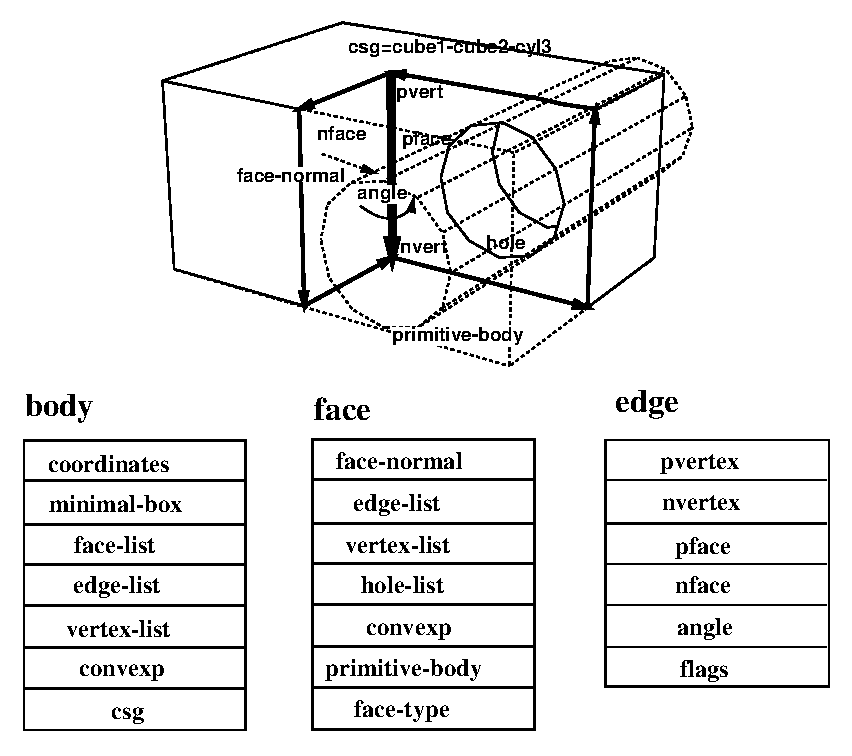
\includegraphics[height=10cm]{fig/beam.ps}
%\epsfile{file=fig/beam.ps,height=10cm}
\end{center}
\caption{頂点とエッジと面の分類}
\end{figure}

\subsection{種々の幾何学関数}

\begin{refdesc}

\funcdesc{vplus}{vector-list}{
{\em vector-list}のすべての要素の合計を実数ベクトルとして
新しく作り、返す。
{\bf v+}との違いは、{\bf vplus}が2つ以上の引数について合計を計算し、
結果のベクトルが指定できない点である。}

\funcdesc{vector-mean}{vector-list}{
{\em vector-list}の平均ベクトルを返す。}

\funcdesc{triangle}{a b c \&optional (normal \#f(0 0 1))}{
{\em a, b, c}は、2次元または3次元の実数ベクトルである。
{\em normal}は、{\em a,b,c}が置かれる平面の正規ベクトルである。
{\bf triangle}は{\em a,b,c}で形作られる三角形の領域の2倍の大きさを返す。
{\em normal}と同じ方向から見たときに{\em a,b,c}が時計方向に回転する
ならば、{\bf triangle}は正である。
言い換えると、もし{\bf triangle}が正ならば、
{\em c}は{\em a-b}の線分の左手側に位置し、
{\em b}は{\em a-c}の右手側に位置している。}

\funcdesc{triangle-normal}{a b c}{
{\em a b c}で定義される三角形に対して垂直方向の正規ベクトルを見つける。}

\funcdesc{vector-angle}{v1 v2 \&optional (normal (v* v1 v2))}{
2つのベクトルの角度を計算する。
これは次の式であらわされる{\tt atan(normal$\cdot$(v1$\times$v2), v1$\cdot$v2)}。
{\em v1,v2}と{\em normal}は正規ベクトルでなければならない。
{\em normal}が与えられないとき、{\em v1,v2}の共通垂線の正規ベクトルが
使用される。この場合、結果は$0$から$\pi$までの範囲の正の角度になる。
符号付きの角度を得るためには、{\em normal}を指定しなければならない。}

\funcdesc{face-normal-vector}{vertices}{
同じ平面の上にあるベクトルのリストから面の正規化ベクトルを計算する。}

\funcdesc{farthest}{p points}{
3次元ベクトルのリスト{\em points}の中から{\em p}より最も遠い点を捜す。}

\funcdesc{farthest-pair}{points}{
3次元ベクトルのリスト{\em points}からもっとも遠い点の組を
捜す。}

\funcdesc{maxindex}{3D-floatvec}{
{\em 3D-floatvec}の3つの要素の中で絶対値が最大の要素の位置を捜す。}

\funcdesc{random-vector}{\&optional (range 1.0)}{
3次元デカルト空間の中で同次的に分散されるランダムベクトルを発生する。}

\funcdesc{random-normalized-vector}{\&optional (range 1.0)}{
3次元の正規化ランダムベクトルを返す。}

\funcdesc{random-vectors}{count range}{
{\em range}の大きさのランダムベクトルを{\em count}個つくり、そのリストを返す。}

\funcdesc{line-intersection}{p1 p2 p3 p4}{
{\em p1, p2, p3, p4}は、すべて2次元以上の実数ベクトルである。
{\em p1-p2}と{\em p3-p4}が平面上の2つの線分として定義される。
{\bf line-intersection}は、これらの2つの線分の交差する点のパラメータ(線分に置ける
交点の位置の比率)を2要素のリストで返す。3次元で使用するとき、
{\em p1, p2, p3, p4}は共通平面内になければならない。}

\funcdesc{collinear-p}{p1 p2 p3 \&optional tolerance}{
{\em p1, p2, p3}は、すべて3次元の実数ベクトルで3つの点を表現している。
{\bf collinear-p}は、もし{\tt $\Vert$((p2$-$p1)$\times$(p3$-$p1))$\Vert$}が
{\tt *coplanar-threshold*}より小さければ、{\em p1-p3}の線分の上に
{\em p2}を投影したときのパラメータを返す。そうでなければ、NILを返す。}

\funcdesc{find-coplanar-vertices}{p1 p2 p3 vlist}{
{\em p1, p2, p3}は、3次元の実数ベクトルで、この3つのベクトルから平面を表現している。
{\bf find-coplanar-vertices}は、その平面内にある点を
{\em vlist}の中から捜す。}

\funcdesc{find-connecting-edge}{vertex edgelist}{
{\em vertex}に接続された{\em edgelist}の中からエッジを捜す。}

\funcdesc{make-vertex-edge-htab}{bodfacs}{
{\em bodfacs}は、{\bf body}あるいは{\bf face}のリストである。
{\bf make-vertex-edge-htab}は、{\em bodfacs}の中の頂点を抽出し、それに接続されるエッジの検索ができる
ハッシュテーブルを作る。}

\funcdesc{left-points}{points p1 p2 normal}{
{\em points, p1, p2}は、正規化ベクトル{\em normal}で表現される
平面内にあるものと仮定する。
{\bf left-points}は、{\em p1, p2}間の線分の左側に置かれている点を
{\em points}の中から捜し、集める。}

\funcdesc{right-points}{points p1 p2 normal}{
{\em points, p1, p2}は、正規化ベクトル{\em normal}で表現される
平面内にあるものと仮定する。
{\bf right-points}は、{\em p1, p2}間の線分の右側に置かれている点を
{\em points}の中から捜し、集める。}

\funcdesc{left-most-point}{points p1 p2 normal}{
{\em points, p1, p2}は、正規化ベクトル{\em normal}で表現される
平面内にあるものと仮定する。
{\bf left-most-points}は、{\em p1, p2}で決定される線分の左側に置かれている点を
{\em points}の中から捜し、その中でもっとも遠い点を返す。}

\funcdesc{right-most-point}{points p1 p2 normal}{
{\em points, p1, p2}は、正規化ベクトル{\em normal}で表現される
平面内にあるものと仮定する。
{\bf right-most-points}は、{\em p1, p2}で決定される線分の右側に置かれている点を
{\em points}の中から捜し、その中でもっとも遠い点を返す。}

\funcdesc{eps=}{num1 num2 [(tolerance *epsilon*)]}{
2つの実数{\em num1}と{\em num2}を比較して、{\em torelance}の誤差範囲内で
等しいかどうかを返す。}
\funcdesc{eps$<$}{num1 num2 [(tolerance *epsilon*)]}{
{\em num1}が明らかに{\em num2}よりも小さいときTを返す。すなわち、
{\tt num1$<$num2-tolerance}である。}
\funcdesc{eps$<=$}{num1 num2 [(tolerance *epsilon*)]}{
{\em num1}が多分{\em num2}よりも小さいときあるいは等しいときTを返す。すなわち、
{\tt num1$<$num2+tolerance}である。}
\funcdesc{eps$>$}{num1 num2 [(tolerance *epsilon*)]}{
{\em num1}が明らかに{\em num2}よりも大きいときTを返す。すなわち、
{\tt num1$>$num2+tolerance}である。}
\funcdesc{eps$>=$}{num1 num2 [(tolerance *epsilon*)]}{
{\em num1}が多分{\em num2}よりも大きいときあるいは等しいときTを返す。すなわち、
{\tt num1$>$num2-tolerance}である。}


\classdesc{bounding-box}{object}{(minpoint maxpoint)}
{xy-,yz-やzx-平面に平行な面を境界とする最小の四角柱を定義する。
{\bf bounding-box}は、初期に与えられるベクトルの次元によって、
どんな次元でも使用することができる。
{\bf bounding-box}は、surrounding-boxの名前で定義されていた。}

\methoddesc{:box}{}{この{\bf bounding-box}のオブジェクト自身を返す。}
\methoddesc{:volume}{}{この{\bf bounding-box}の体積を返す。}
\methoddesc{:grow}{rate}{
この{\bf bounding-box}のサイズを{\em rate}率で増加または減少させる。
{\em rate}が0.01のとき、1\%拡大される。}
\methoddesc{:inner}{point}{
{\em point}がこの{\bf bounding-box}内にあればTを返し、
そうでないときはNILを返す。}
\methoddesc{:intersection}{box2 \&optional tolerance}{
この{\bf bounding-box}と{\em box2}との共通{\tt bounding-box}を返す。
もし、{\em torelance}が与えられたならば、この{\bf box}はその誤差で拡大される。
もし、共通部分がなければ、NILを返す。}
\methoddesc{:union}{box2}{
この{\bf bounding-box}と{\em box2}を結合した{\tt bounding-box}を返す。}
\methoddesc{:intersectionp}{box2}{
この{\bf bounding-box}と{\em box2}との間に共通領域があればTを返し、
そうでなければNILを返す。
このメソッドは、{\bf :intersection}よりも速い。なぜなら、新しい
{\bf bounding-box}のインスタンスを作らないためである。}
\methoddesc{:extreme-point}{direction}{
この{\bf bounding-box}の8つの頂点の中で、{\em direction}との内積が最大のものを
返す。}
\methoddesc{:corners}{}{
この{\bf bounding-box}のすべての頂点のリストを返す。
もし、この{\bf box}が2次元であれば、4点が返される。
同様に3次元の場合、8点が返される。}
\methoddesc{:below}{box2 \&optional (direction \#(0 0 1)}{
この{\bf bounding-box}が{\em box2}に対して{\em direction}の示すベクトル
の下の方向にあればTを返す。
この{\bf boundign-box}が{\em direction}の方向に動かされるとき、
2つのboxに共通部分でできるかどうかをチェックするために使用される。}
\methoddesc{:body}{}{
この{\bf bounding-box}によって内包される立方体を表現する
{\bf body}を返す。}
\methoddesc{:init}{vlist \&optional tolerance}{
{\tt minpoint}と{\tt maxpoint}スロットを{\em vlist}から設定する。
もし、{\em torelance}が指定されたなら、この{\bf bounding-box}は
その量で増大される。}

\funcdesc{make-bounding-box}{points [tolerance]}{
{\em points}のリストの中から最小と最大の座標値を見つけ、
{\tt bounding-box}のインスタンスを作る。}
\funcdesc{bounding-box-union}{boxes [tolerance *contact-threshold*]}{
{\em boxes}の結合で表現されるbounding-boxのインスタンスを作る。
その結果は、{\em tolerance}によって拡張される。}
\funcdesc{bounding-box-intersection}{boxes [tolerance *contact-threshold*]}{
{\em boxes}の共通領域を表現するbounding-boxのインスタンスを作る。
その結果は、{\em tolerance}によって拡張される。}
\end{refdesc}

\newpage
\subsection{線とエッジ}

頂点の順番やエッジの順番の向きは、{\bf body}を外から見たときに反時計方向
に整列するように定義される。
{\tt pvertex}や{\tt nvertex}や{\tt pface}や{\tt nface}は、
{\tt pface}が外から見たときエッジの左側に位置しているとき、
{\tt pvertex}から{\tt nvertex}に向かう方向にエッジを定義する。

\begin{refdesc}

\classdesc{line}{propertied-object}
{((pvert :type floatvector)
(nvert :type floatvector))}{
{\tt pvert}と{\tt nvert}の上を通る線分を定義する。
線分は、{\em pvert}から{\em nvert}に向かう方向を持つ。
{\tt t $\cdot$ pvert +(1-t)nvert}}

\methoddesc{:vertices}{}{{\tt pvert}と{\tt nvert}のリストを返す。}

\methoddesc{:point}{p}{
この線分の上で{\em p}パラメータで示される位置の3次元のベクトルを返す。
{\tt p $\cdot$ pvert + (1-p)nvert}}
\methoddesc{:parameter}{point}{
この線分の上の{\em point}に対するパラメータを計算する。
これは、{\bf :point}メソッドの逆メソッドである。}
\methoddesc{:direction}{}{
{\tt pvert}から{\tt nvert}へ向かう正規化ベクトルを返す。}
\methoddesc{:end-point}{v}{
この線分の他の端点を返す。すなわち、
もし{\em v}が{\tt pvert}に等しいとき、{\tt nvert}を返す。
もし{\em v}が{\tt nvert}に等しいとき、{\tt pvert}を返す。
それ以外のとき、NILを返す。}

\methoddesc{:box}{}{この線分の{\bf bounding-box}を作成し、返す。}
\methoddesc{:boxtest}{box}{
{\em box}とこの線分の{\bf bounding-box}の共通部分をチェックする。}
\methoddesc{:length}{}{この線分の長さを返す。}
\methoddesc{:distance}{point-or-line}{
この線分と{\em point-or-line}の間の距離を返す。
もし点からこの線分におろした垂線の足が
{\tt pvert}と{\tt nvert}の間になければ、
最も近い端点までの距離を返す。
このメソッドを使うことにより、2つの線分の間の距離を計算することができるため、
2つの円柱の間の干渉をテストすることができる。}

\methoddesc{:foot}{point}{
{\em point}からこの線分へおろした垂線の足である点を示すパラメータ
を見つける。}
\methoddesc{:common-perpendicular}{l}{
この線分と{\em l}とに垂直な線分を見つけ、2つの3次元ベクトルのリスト
として返す。
2つの線分が平行で共通な垂線が一意に決定できないとき、{\tt :parallel}を返す。}
\methoddesc{:project}{plane}{
{\em plane}に{\tt pvert}と{\tt nvert}を投影した2つの点のリストを返す。}
\methoddesc{:collinear-point}{point \&optional (tolerance *coplanar-threshold*)}{
{\bf collinear-p}を用いて{\em torelance}の誤差範囲内で{\em point}がこの線分と
一直線上にあるかどうかをチェックする。
もし、{\em point}がこの線分と一直線上にあるとき、その線分のその点に
対するパラメータを返す。そうでなければ、NILを返す。}
\methoddesc{:on-line-point}{point \&optional (tolerance *coplanar-threshold*)}{
{\em point}がこの線分と一直線上にあり、{\tt pvert}と{\tt nvert}との間に
あるかどうかをチェックする。}
\methoddesc{:collinear-line}{ln \&optional (tolerance *coplanar-threshold*)}{
{\em ln}がこの線分と共通線上にあるとき、すなわち{\em ln}の両端がこの線分上に
あるときTを返し、そうでないときNILを返す。}
\methoddesc{:coplanar}{ln \&optional (tolerance *coplanar-threshold*)}{
{\em ln}とこの線分が共通平面上にあるかどうかをチェックする。
この線分の両端と{\em ln}の1つの端点で平面が定義される。
もし、{\em ln}の他の端点がその平面上にあるとき、Tを返す。
そうでなければ、NILを返す。}
\methoddesc{:intersection}{ln}{
{\em ln}は、この線分と共通平面上にあるとする。
{\bf :intersection}は、これら2つの線分の交点に対する2つのパラメータの
リストを返す。
パラメータは0から1までの実数である。これは、両端で区切られた
線分の内分点を示す。2つの線が平行であるときNILを返す。}
\methoddesc{:intersect-line}{ln}{
{\em ln}は、この線分と共通平面上にあるとする。
交点のパラメータが{\tt :parallel, :collinear}や{\tt :intersect}のような
シンボル情報と共に返される。}

\classdesc{edge}{line}
{(pface nface \\
 \> (angle :type float) \\
 \> (flags :type integer))}
{2つの面の間の交差線分として定義されるエッジを表現する。
{\tt pface}と{\tt nface}がスロットの中に定義されているが、
それらの解釈はこのエッジの方向によって相対的に決まる。
例えば、このエッジが{\tt pvert}から{\tt nvert}に向かっていると
考えたとき、{\tt pface}が正しいpfaceを表現している。
そのため、{\bf :pface}や{\bf :nface}メソッドで適当な面を選択するためには、
pvertとnvertの解釈を与えなければならない。
}

\funcdesc{make-line}{point1 point2}{
{\em point1}を{\tt pvert}とし、{\em point2}を{\tt nvert}とする
{\bf line}のインスタンスを作る。}

\methoddesc{:pvertex}{pf}{
{\em pf}をこのエッジの{\tt pface}とみなした{\tt pvertex}を返す。}

\methoddesc{:nvertex}{pf}{
{\em pf}をこのエッジの{\tt pface}とみなした{\tt nvertex}を返す。}

\methoddesc{:body}{}{このエッジを定義する{\bf body}オブジェクトを返す。}
\methoddesc{:pface}{pv nv}{仮想的に{\em pv}と{\em nv}をこのエッジの
pvertとnvertに解釈したときのpfaceを返す。}
\methoddesc{:nface}{pv nv}{仮想的に{\em pv}と{\em nv}をこのエッジの
pvertとnvertに解釈したときのnfaceを返す。}
\methoddesc{:binormal}{aface}{
このエッジと{\em aface}の正規化ベクトルに垂直な方向ベクトルを見つける。}
\methoddesc{:angle}{}{
このエッジでつながった2つの面の間の角度を返す。}
\methoddesc{:set-angle}{}{
このエッジでつながった2つの面の間の角度を計算し、
それを{\tt angle}スロットに置く。}

\metdesc{:invert}{}
\methoddesc{:set-face}{pv nv f}{
{\em f}を{\tt pface}とし、{\em pv}を{\tt pvertex}とし、{\em nv}を
{\tt nvertex}として設定する。
このメソッドは、このエッジの{\tt pface}あるいは{\tt nface}を変更することに
注意すること。}

\methoddesc{:contourp}{ viewpoint}{
もし、このエッジが輪郭エッジであれば、すなわち、このエッジの{\tt pface}
あるいは{\tt nface}のどちらかが{\em viewpoint}から見え、もう一方が
見えないならTを返す。}

\methoddesc{:approximated-p}{}{
このエッジが円柱の側面のような曲面を表現するための近似エッジであるならば、
Tを返す。
近似エッジは部分直線で曲線を表現するのに必要である。
%If edges are defined to exist where the curvature changes non-continuously,
%these approximated edges should not exist.
}

\methoddesc{:set-approximated-flag}{\&optional (threshold 0.7)}{
Euslispでは、どんな曲面もたくさんの平面で近似される。
{\tt flags}のLSBは、このエッジの両側の面が曲面であるかどうかを
示すために使用される。

もし、2つの面の間の角度が{\em threshold}より大きいなら、
{\bf :set-approximated-flag}は、このフラグをTに設定する。}

\metdesc{:init}{\&key :pface :nface :pvertex :nvertex}

\end{refdesc}

\newpage
\subsection{平面と面}

{\bf plane}オブジェクトは、その平面の正規化ベクトルと座標原点から平面までの
距離で表現される。
2対の正規化ベクトルと距離が{\bf plane}オブジェクトに記録される。
1つは、変換後の現状を表現し、もう1つが平面を定義したときの
正規化ベクトルと距離を表現する。

\begin{refdesc}

\classdesc{plane}{propertied-object}
{((normal :type float-vector) \\
\> (distance :float))}
{平面方程式を定義する。平面は境界がなく、無限に広がっているものとする。}

\methoddesc{:normal}{}{
この平面の正規化ベクトルを返す。}
\methoddesc{:distance}{ point}{
この平面と{\em point}との間の距離を計算する。}
\methoddesc{:coplanar-point}{point}{
もし、{\em point}がこの平面の上に置かれているならTを返す。}
\methoddesc{:coplanar-line}{line}{
もし、{\em line}がこの平面の上に置かれているなら、Tを返す。}

\methoddesc{:intersection}{ point1 point2}{
{\em point1}と{\em point2}を端点とする線分とこの平面との交点
を計算する。その線分の上の交点に対するパラメータを返す。
もし、線分とこの平面が平行であるなら、{\tt :parallel}を返す。}
\methoddesc{:intersection-edge}{edge}{
この平面と{\em point1}と{\em point2}で表現される線分あるいはエッジとの
交点のパラメータを返す。}
\methoddesc{:foot}{point}{
この平面上に{\em point}を直角に投影した位置の3次元ベクトルを返す。}

\methoddesc{:init}{normal point}{
{\em point}を通り{\em normal}を面の正規化ベクトルとする平面を定義する。
{\em normal}は、正規化されていなければならない。$|normal|=1$}

\classdesc{polygon}{plane}
{(convexp edges vertices \\
\> (model-normal float-vector) \\
\> (model-distance :float))\\}{
{\bf polygon}は、平面の上の輪で表現される。
{\tt convexp}は、その輪が凸面であるかどうかを示す論理フラグである。
{\tt edges}は、この輪の輪郭や頂点のリストである{\tt vertices}で
形成されるエッジのリストである。}

\methoddesc{:box}{\&optional tolerance}{
この多角形のための{\bf bounding-box}を返す。}
\methoddesc{:boxtest}{box2 \&optional tolerance}{
この多角形のための{\bf bounding-box}を作成し,
その{\bf boundign-box}と{\em box2}との共通領域を返す。
もし,共通領域がなかった場合,NILを返す。}
\methoddesc{:edges}{}{
この多角形のエッジのリストを返す。
そのリストは,この平面の正規化ベクトルに沿ってその多角形を見たとき,
時計方向の順番になっている。
もし,正規化ベクトルをねじと考えると,そのエッジは
ねじを入れる方向に回転させる向きの順番になっている。
多角形または面が立体オブジェクトの面を表現するために使用されているとき,
その正規化ベクトルはその立体の外側に向かっている。
多角形をそのオブジェクトの外側から見たとき,エッジは
反時計方向の順番になっている。}
\methoddesc{:edge}{n}
{エッジの{\em n}番目の要素を返す。}
\methoddesc{:vertices}{}{
この多角形の頂点をエッジと同じ順番にならべたものを返す。
最初の頂点は,そのリストの最後に重複してコピーされているため,
そのリストは実際の頂点の数より1だけ長くなっていることに注意すること。
これは,頂点のリストを用いてエッジへの変換を簡単にするためである。}
\methoddesc{:vertex}{n}
{頂点の{\em n}番目の要素を返す。}
\methoddesc{:insidep}{point \&optional (tolerance *epsilon*)}{
この領域に対して相対的に置かれた{\em point}の位置にしたがって
{\tt :inside},{\tt :outside}あるいは{\tt :border}を返す。}
\methoddesc{:intersect-point-vector}{ point vnorm}{
{\em point}と正規化方向ベクトル{\em vnorm}によって定義される
擬似線分との交点を計算する。}
\methoddesc{:intersect-line}{p1 p2}{
{\em p1}と{\em p2}で指定される線分との交点を計算する。
その結果は、交点がなければNILを返し,交点があればその交点の位置の
パラメータのリストを返す。}
\methoddesc{:intersect-edge}{edge}{
{\em edge}で指定される線分との交点を計算する。
その結果は,交点がなければNILを返し、交点があれば
交点の位置のパラメータのリストを返す。}
\methoddesc{:intersect-face}{aregion}{
もし,この領域が{\em aregion}と交差しているなら,Tを返す。}
\metdesc{:transform-normal}{}
\methoddesc{:reset-normal}{}{
この多角形の現在の{\tt vertices}リストから面の正規化ベクトルを再計算する。}
\metdesc{:invert}{}
\methoddesc{:area}{}{この領域の面積を返す。}
\metdesc{:init}{\&key :vertices :edges :normal :distance}

\classdesc{face}{polygon}
{(holes mbody primitive-face id)}{穴を持った面を定義する。
{\em mbody}と{\em type}は、基本bodyとbody内の面の属性{\tt (:top, :bottom, :side)}
を表現する。}

\metdesc{:all-edges}{}
\methoddesc{:all-vertices}{}{
この面および内部ループ(穴)の輪郭のエッジあるいは頂点をすべて返す。
{\bf :edges}と{\bf :verticies}メソッドは,
輪郭を構成するエッジと頂点のみを返す。}
\methoddesc{:insidep}{point}{
{\em point}がこの面の内部にあるかどうかを決定する。
もし{\em point}がこの面の外側の輪郭の中にあり,どれかの穴の
範囲内にあるならば,外側として分類される。}
\methoddesc{:area}{}{
この面の面積を返す。
これは,外側のエッジで囲まれる面積から穴の面積を引いたものである。}
\methoddesc{:centroid}{ \&optional point}{
この面の重心を表現する実数と実数ベクトルのリストを返す。
もし,{\em point}が与えられないならば,最初の数はこの多角形の
面積を表わし,2番目のベクトルがこの多角形の重心の位置を示す。
もし,{\em point}が与えられたならば,この多角形を底面としその点を頂点
とするような多角錐を考え,その体積と重心のベクトルを返す。}
\methoddesc{:invert}{ }{
この面の向きをひっくり返す。
正規化ベクトルが逆方向とされ,エッジループの順番も反転される。}
\methoddesc{:enter-hole}{hole}{
この面に穴{\em hole}を加える。}
\methoddesc{:primitive-body}{}{
この面を定義する基本{\bf body}を返す。}
\methoddesc{:id}{}{
{\tt (:bottom), (:top)}や{\tt (:side seq-no.)}の中の1つを返す。}
\methoddesc{:face-id}{}{
基本{\bf body}の型とこの面の型をリストで返す。
例えば,円柱の側面は
{\tt ((:cylinder {\em radius height segments}) :side {\em id})}を返す。}
\methoddesc{:body-type}{}{
この面を定義する基本{\bf body}を返す。}
\metdesc{:init}{ \&key :normal :distance :edges :vertices :holes}

\classdesc{hole}{polygon}
{(myface)}
{穴は,面の内部ループを表現する多角形である。{\bf face}のオブジェクトは、
自分の{\tt holes}スロット
の中に{\bf hole}のリストを持っている。}

\methoddesc{:face}{}
{この{\bf hole}を含む面を返す。}
\methoddesc{:enter-face}{face}{
この{\bf hole}を囲んでいる面{\em face}へリンクを作る。
このメソッドは、{\bf face}クラスの{\tt :enter-hole}メソッドと共に
使用されるものである。}
\metdesc{:init}{ \&key :normal :distance :edges :vertices :face}

\newpage
\subsection{立体(body)}

\classdesc{body}{cascaded-coords}
{(faces edges vertices model-vertices
 box convexp evertedp csg)}{3次元形状を定義する。}

\methoddesc{:magnify}{rate}{
この{\bf body}のサイズを{\em rate}で変更する。拡大は,{\tt csg}リストの中に
記録される。}

\methoddesc{:translate-vertices}{ vector}{
モデルの頂点を相対移動する。{\em vector}はローカル座標系で与えられなければならない。
変換は{\tt csg}リストに記録される。}

\methoddesc{:rotate-vertices}{ angle axis}{
モデルの頂点を{\em axis}軸回りに{\em angle}ラジアン回転させる。
回転は{\tt csg}リストに記録される。}
\metdesc{:reset-model-vertices}{}
\methoddesc{:newcoords}{rot \&optional pos}{
座標系を{\em rot}や{\em pos}を用いて変更する。
{\em pos}が省略された時は{\em newrot}にはcoordinatesのインスタンスを与える。}
\methoddesc{:vertices}{}{この{\bf body}のすべての頂点のリストを返す。}
\methoddesc{:edges}{}{この{\bf body}のすべてのエッジのリストを返す。}
\methoddesc{:faces}{}{
この{\bf body}を構成するすべての面のリストを返す。}
\methoddesc{:box}{}{この{\bf body}の{\bf bounding-box}を返す。}
\methoddesc{:Euler}{}{
この{\bf body}のオイラー数を計算する。これは,
{\tt faces+vertices$-$edges$-$2$-$holes}である。
これは,{\tt $-$2rings}と等しくなるべきである。}
\methoddesc{:perimeter}{}{
すべてのエッジの長さの合計を返す。}
\methoddesc{:volume}{ \&optional (reference-point \#f(0 0 0))}{
この{\bf body}の体積を返す。}
\methoddesc{:centroid}{ \&optional (point \#f(0 0 0)}{
この{\bf body}が均質な立体と仮定し,重心の位置を返す。}
\metdesc{:possibly-interfering-faces}{box}
\methoddesc{:common-box}{body}{
この{\bf body}と他の{\em body}の共通な最小の{\bf box}を返す。
もし,2つの{\bf body}が干渉しているならば,その交差部分は
この共通{\bf box}の中に存在するはずである。}
\methoddesc{:insidep}{ point}{
もし,{\em point}がこの{\bf body}に属するなら,{\tt :inside}を返す。
もし,{\em point}がこの{\bf body}の表面上にある場合,{\tt :border}を返す。
そうでなければ,{\tt :outside}を返す。}

\methoddesc{:intersect-face}{face}{
もし,この{\bf body}の面と{\em face}の間に干渉がある場合,Tを返す。}
\methoddesc{:intersectp}{body}{
この{\bf body}と他の{\em body}との間の交差部分を返す。}
\methoddesc{:evert}{}{すべての面とエッジの方向を反転させる。
そのため,この{\bf body}の内部は外部になる。}
\methoddesc{:faces-intersect-with-point-vector}{point direction}{
{\em point}から{\em direction}の方向に伸びるベクトルと交差する面をすべて集める。}
\methoddesc{:distance}{target}{
{\em target}は,実数ベクトルあるいは平面オブジェクトである。
{\bf :distance}メソッドは,{\em target}から最も近い面を見つけ,
その面と距離のリストを返す。}
\methoddesc{:csg}{}{
{\bf body}が構築された履歴である{\tt csg}スロットを返す。}
\methoddesc{:primitive-body}{ }{
この{\bf body}を構築する基本{\bf body}のリストを返す。}
\methoddesc{:primitive-body-p}{}{もし,この{\bf body}が\ref{primitive-body-creation}
節で示される関数の内の1つから作られた基本{\bf body}であるなら,Tを返す。}
\methoddesc{:creation-form}{}{
この{\bf body}を作るためのLisp表現を返す。}
\methoddesc{:body-type}{}{
もし,この{\bf body}が基本{\bf body}あるいはこの{\bf body}の表現が複雑(に構成された)
{\bf body}なら,作成パラメータのリストを返す。}
\methoddesc{:primitive-groups}{}{
2つの要素をもつリストを返す。
最初の要素は,この{\bf body}を構成するために追加(body+)された基本{\bf body}
のリストである。次の要素は,差し引かれた基本{\bf body}のリストである。}
\methoddesc{:get-face}{body \&optional face id}{
{\em body}は,この{\bf body}を構成している{\bf body}のインスタンスであり,
基本{\bf body}型の1つである。例えば,{\tt :cube, :prism, :cone, :solid-of-resolution}などか
あるいはNILである。
もし,{\em face}も{\em id}も与えられないならば,{\em body}に一致する面をすべて返す。
もし,{\em face}が与えられたなら,その上にフィルターが実行される。
{\em face}は,{\tt :top},{\tt :bottom}と{\tt :side}の内の1つでなければならない。
{\tt (send abody :get-face :cylinder :top)}は,{\tt abody}を構成する円柱の上面すべてを返す。
もし,{\em face}が{\tt :side}なら,{\em id}で番号付けされた面を取り出すことができる。
{\tt (send abody nil :side 2)}は,{\em id}が0から始まるため,{\tt abody}を構成する
{\bf body}の側面から3番目の面をすべて返す。}
\methoddesc{:init}{ \&key :faces :edges :vertices}{
{\em :faces}よりこの{\bf body}を初期化する。
{\em :faces}は,必要な引き数である。
{\em :faces},{\em :edges}と{\em :vertices}は完全な立体モデルを定義するために
矛盾のない関係を持っていなければならないので,矛盾した引き数でこのメソッドを
呼び出すことは,意味の無いことである。
{\bf body}を作るために,\ref{primitive-body-creation}節で書いている基本{\bf body}の作成関数と
\ref{BodyComposition}節の{\bf body}合成関数を使用する。}
\methoddesc{:constraint}{b}{この{\bf body}が{\em b}に接触しているとき,
この{\bf body}の拘束を返す。このメソッドの詳細な説明は\ref{Contact}節を参照すること。}


\end{refdesc}
\newpage
\subsection{\label{primitive-body-creation}基本bodyの作成関数}

\begin{refdesc}

\funcdesc{make-plane}{\&key :normal :point :distance}{
{\em point}を通り,{\em normal}の方向を向いた{\bf plane}オブジェクトを作る。
{\em point}を与える代わり{\em distance}を指定することもできる。}

\vardesc{*xy-plane*}{\hspace{0mm}}
\vardesc{*yz-plane*}{\hspace{0mm}}
\vardesc{*zx-plane*}{\hspace{0mm}}

\begin{figure}
\begin{center}
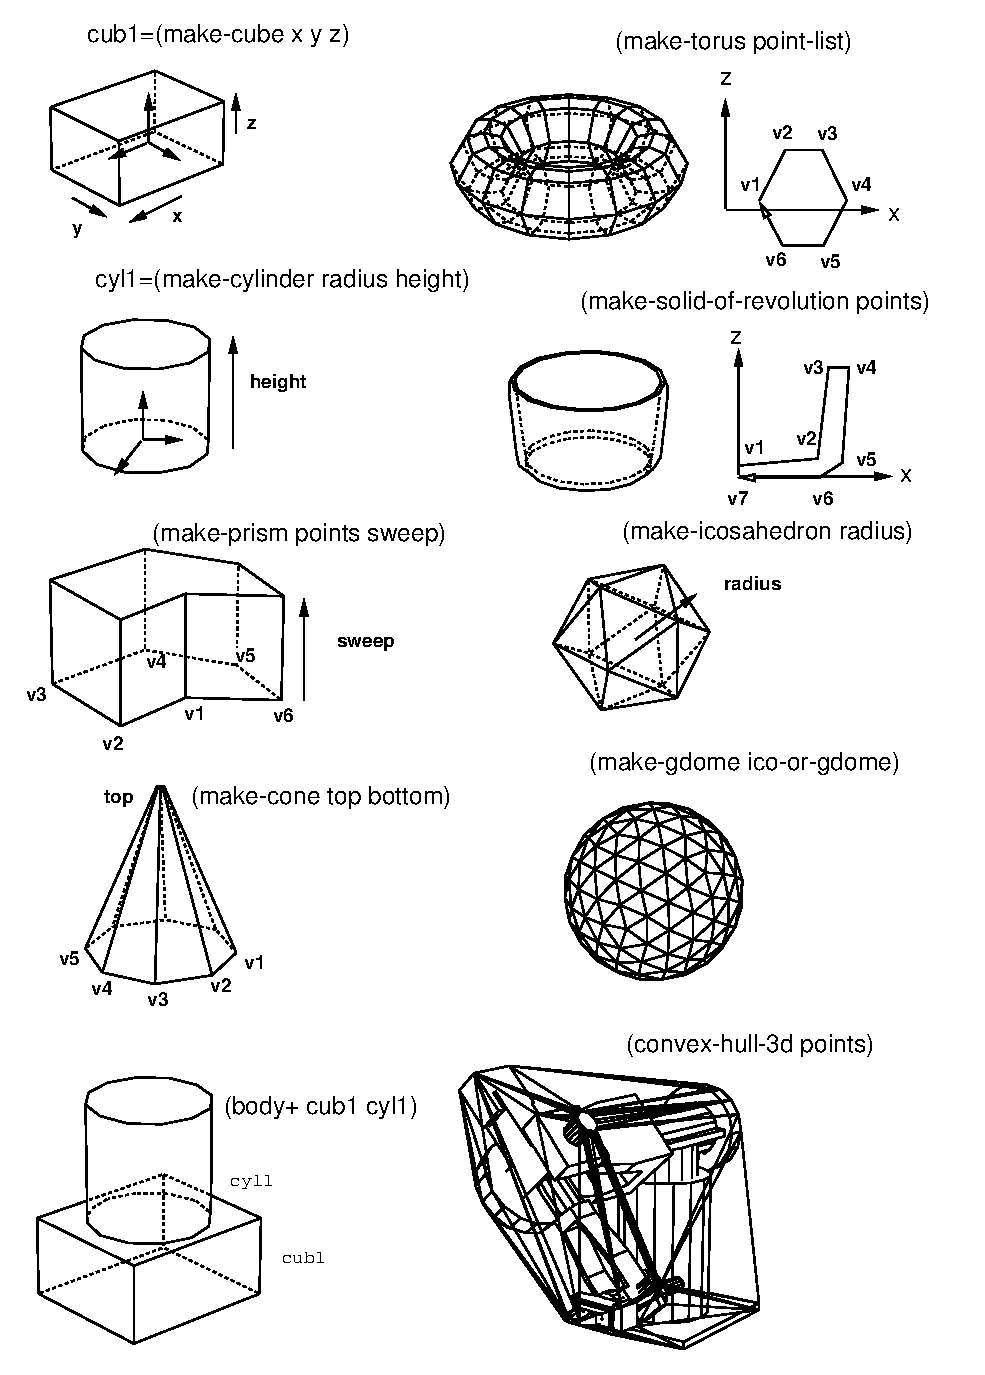
\includegraphics[height=19cm]{fig/fig1.ps}
%\epsfile{file=fig/fig1.ps,height=19cm}
\end{center}
\caption{基本body}
\end{figure}

\funcdesc{make-cube}{xsize ysize zsize \&key :name :color}{
x,y,z軸の方向に大きさが{\em xsize},{\em ysize},{\em zsize}である,直方体を作る。
この直方体の原点は{\bf body}の中心に置かれる。}

\funcdesc{make-prism}{bottom-points sweep-vector \&key :name :color}{
{\em sweep-vector}に沿った{\em bottom-points}により定義される
形状を積み上げることにより角柱を作る。
もし、{\em sweep-vector}が実数ベクトルでなく数字であれば、$z$方向の
角柱の高さとして扱われる。
{\em bottom-points}は,この{\bf body}の底面を定義する順番になっていなければならない。
例えば,
 {\tt (make-prism '(\#f(1 1 0) \#f(1 -1 0) \#f(-1 -1 0) \#f(-1 1 0)) 2.0)}
は,高さ2.0の直方体を作る。}

\funcdesc{make-cylinder}{radius height \&key (:segments 12) :name :color}{
半径{\em radius}と高さ{\em height}で指定される円柱を作る。
底面は,xy-平面に定義され,座標系の原点は底面の中心に置かれる。}

\funcdesc{make-cone}{top bottom \&key (:segments 16) :color :name}{
頂点が{\em top}で底面が{\em bottom}である角錐を作る。
{\em top}は,3次元ベクトルである。
{\em bottom}は,底面の頂点のリストあるいは半径である。
もし,頂点のリストなら,順番を慎重にしなさい。
%%% change 2004.12.14 \verb+ (make-cone \#f(0 0 10) (list \#f(10 0 0) \#f(0 10 0) \#f(-10 0 0)
%%% change 2004.12.14 \#f(0 -10 0)))+ は,正方形の底面を持つ四角錐を作る。}
\verb~ (make-cone \#f(0 0 10) (list \#f(10 0 0) \#f(0 10 0) \#f(-10 0 0)
\#f(0 -10 0)))~ は,正方形の底面を持つ四角錐を作る。}

\funcdesc{make-solid-of-revolution}{points \&key (:segments 16) :name :color}{
{\em points}は,z軸まわりの時計方向に回転される。
もし、{\em points}のリストの2つの端点がz軸上に置かれてないならば,
曲面を作る。したがって,
{\tt (make-solid-of-revolution '(\#f(0 0 1) \#f(1 0 0)))}
は、円錐を作り、
{\tt (make-solid-of-revolution '(\#f(1 0 1) \#f(1 0 0)))}
は、円柱を作る。
{\em points}は、順番が重要であり、$z$軸の高い方から低い方へ
整列しておくことが望まれる。}

\funcdesc{make-torus}{points \&key (:segments 16) :name :color}{
ドーナッツのようなtorus形状を作る。
{\em points}は,断面上の頂点のリストである。}

\funcdesc{make-icosahedron}{\&optional (radius 1.0)}{
正20面体を作る。それぞれの面は正三角形である。}

\funcdesc{make-dodecahedron}{\&optional (radius 1.0)}{
正12面体を作る。それぞれの面は,正五角形である。}

\funcdesc{make-gdome}{abody}{
{\em abody}の三角面を4つの面に小分けすることにより
測地ドームを新しく作る。
{\em abody}は,最初正20面体とすべきである。
それから,{\bf make-gdome}の結果を再帰的に{\bf make-gdome}に与えることができる。
それぞれの呼び出しで,測地ドームの面の数は,4倍に増加する。すなわち,
20, 80, 320, 1280, 5120などになる。}

\begin{quote}
\begin{verbatim}
(setq g0 (make-icosahedron 1.0))        ; 20 facets
(setq g1 (make-gdome g0))               ; 80 facets
(setq g2 (make-gdome g1))               ; 320 facets
...
\end{verbatim}
\end{quote}

\funcdesc{grahamhull}{vertices \&optional (normal \#f(0 0 1))}{
Grahamのアルゴリズムを用いて,2次元上で凸状の覆いを計算する。
{\bf quickhull}よりも遅い。}

\funcdesc{quickhull}{vertices \&optional (normal \#f(0 0 1))}{
2分探索法を用いて2次元上で凸状の覆いを計算する。}

\funcdesc{convex-hull-3d}{vertices}{
gift-wrapping法を用いて3次元上で凸面の覆いを計算する。}
\funcdesc{make-body-from-vertices}{vertices-list}{
矛盾しない順番になっている面のループを定義する頂点のリストから{\bf body}を返す。}

\end{refdesc}

\subsection{\label{BodyComposition}bodyの合成関数}

\begin{refdesc}

\fundesc{face+}{face1 face2}
\funcdesc{face*}{face1 face2}{
{\em face1}と{\em face2}は,3次元上で共通平面上にある。
{\bf face+}は,これらの面の結合を構築し,面のオブジェクトとして返す。
もし,交差領域がないなら,元の2つの面が返される。
{\bf face*}は,これらの面の交差領域を返す。もし,交差領域がなければ,NILを返す。}

\funcdesc{cut-body}{body cutting-plane}{
{\em body}を{\em cutting-plane}で切断し,その切断面に作られる面のリストを返す。}

\fundesc{body+}{body1 body2 \&rest more-bodies}
\fundesc{body-}{body1 body2}
\funcdesc{body*}{body1 body2}{
2つあるいはそれ以上の{\bf body}の和,差あるいは積を計算する。
それぞれのbodyは,{\bf body+, body-, body*}の処理を行う前に
コピーされ,元のbodyは変更されない。
その結果のbodyの新しい座標系の位置・姿勢は,ワールド座標系のものと一致している。
もし,しきい値パラメータ{\tt *coplanar-threshold*},{\tt *contact-threshold*},{\tt *parallel-threshold*}
を正確に設定するなら,2つの{\bf body}が面同士で接触している場合でも
これらの関数は正しく働くであろう。
しかしながら,もし{\bf body}の頂点が他の{\bf body}の頂点あるいは面に接触している場合,
どの処理も失敗する。}

\funcdesc{body/}{body plane}{
{\bf make-plane}で作られた{\bf plane}クラスのインスタンスである{\em plane}で
{\em body}を切断する。新しく作られた{\bf body}が返される。}

\funcdesc{body-interference}{\&rest bodies}{
{\em bodies}の中で1対1の組み合わせにおける干渉をチェックし,
交差している2つの{\bf body}のリストを返す。}

\end{refdesc}

\subsection{座標軸}
{\bf coordinates-axes}クラスは,画面上に表示可能な3次元座標軸を定義する。
それぞれの軸とz軸の頂点の矢印は,{\bf line}オブジェクトで定義される。
このクラスは,{\bf cascaded-coords}を継承しているので,
このクラスのオブジェクトは,{\bf body}のような他の{\bf cascaded-coords}を元とする
オブジェクトに付けることができる。
このオブジェクトは,{\bf body}の座標軸あるいは他の座標の相対座標系を見るために
使用される。

\begin{refdesc}
\classdesc{coordinates-axes}{cascaded-coords}
{(size model-points points lines)}{表示可能な3次元座標軸を定義する。}
\end{refdesc}

\newpage
